\section{Introduction}
Many of the decisions we make are based on recommendations, from either people we know or increasingly recommender system tailored to our preferences. This is necessary, partly due to the amount of information overload we are exposed to in our everyday lives. The recommendations, or more specific in our case, the recommender system, can cut down the number of options to a manageable level and hereby augmenting the decision-making process without forcing a decision.

The problem with the traditional recommender systems is that it typically make recommendations specifically to one person but often these decisions needs to be taken in a social context. Some scenarios where this could be the case is for example selecting an item from among a vast number of options and only knowing ones own preferences, such as selecting a movie on a streaming service, finding a restaurant, or a vacation destination.

One of the problems regarding taking the social context into consideration is that the recommender have to strive for consensus between the people it recommends to. An already complex problem is made even harder by having to solve it for multiple users simultaneously with new rules in play. From here, we will reference to this problem as making a group recommendation.

%Different methods for group recommendations 
When making group recommendations there are two main approaches, namely profile aggregation and recommendation aggregation\cite{recbook:profilvsrec}. The idea behind profile aggregation is to aggregate the users' preferences into a single group profile and make aggregations based on that profile. The other approach is to consider each user and aggregate the recommendations for the individual users into one aggregation that fits the groups preferences. In this paper we have chosen to focus on aggregation recommendations.

%as we want to make the method work for shifting groups and we deem this approach to fit this case best. \note{find source or fitting argument, Lukas: not sure there are any}

%Describe the approach of using top-k lists
As we are going to aggregate the users recommendations we have chosen to only to focus at the top-k part of their recommendations and return a top-k lists as a result. Furthermore, the top-k lists will be ranked with the highest rated item at first position on the list. Throughout the paper we have worked with a $k$ of size 10.

With ranked top-k lists being partial lists, we have selected three types of aggregation list which have shown good results when used for aggregating search engine results within the information retrieval domain for partial lists. The methods we are using is Borda Count, Markov Chain, and Spearman's Footrule\cite{Masthoff2004, rank:aggregation}. We also implemented an Average aggregation method as a control algorithm.

%Problem regarding evaluation of the aggregation results
Having the group recommendations we are faced with the challenge of evaluating the result as there are no dataset supplying us with a ground truth for group recommendation. However, from the information retrieval domain, we can find measures to evaluate the quality of queries that can be used to evaluate the quality of a partial list of recommendations and there are many datasets available for individual recommendations.

%Lukas
%As it is no longer of question of should the computers be involved when humans make decisions but how.

%Recommender systems can strengthen decision making without taking away the final choice from humans. This opens the 

%For making a decision, Edwards et al provide a 19 step guide for picking the option with the highest utility, and they argue that the problem for a user would be in picking from among the many options presented, also known as information overload\cite{Edwards2001}.

%Recommender systems deal with reducing the problem for a user to a manageable amount of choices. Given a user's preferences, a good recommender system can narrow down the number of choices to a manageable level.

%However when the problem area is expanded to include multiple users in need of a single choice, the problem area is two-fold, as the many individual preferences must be aligned into that of a single recommendation.

%The recommender system is doubly challenged as while a single user can navigate the given recommendations and reflect on each item for the best optimal choice, a group will have a hard time making insightful decisions about items they lack the shared information of the group to comment on.

\subsection{Composition of a Group Recommender}
As we are going to aggregate recommendations we implemented it as can be seen in Figure \ref{fig:composition}. A dataset will provide for us to make some individual recommendations for users arranged into groups for later testing. The next step is where we want to make a contribution and we are trying several different approaches which we evaluate on.
%As we take the aspect of aggregating recommendations the group recommendation system will consist of two parts namely an individual recommender and an aggregation method. \note{need some extension and probably an illustration}
\begin{figure}
\centering
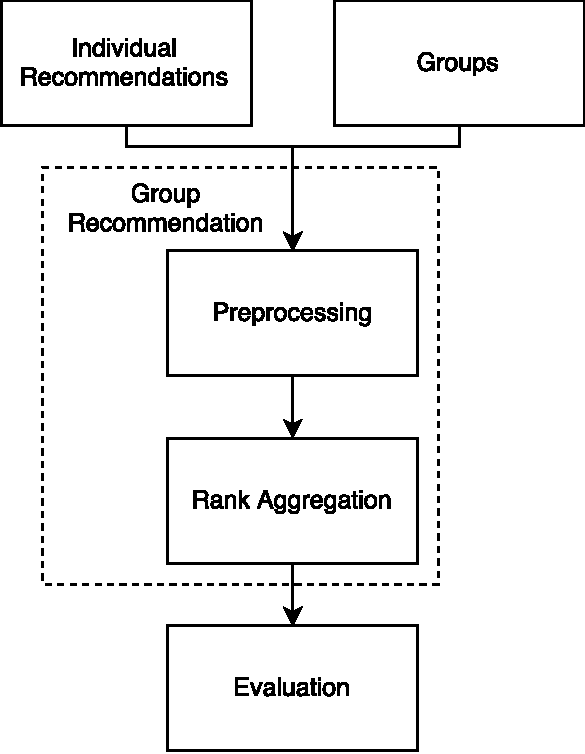
\includegraphics[scale=.4]{graphics/composition}
\caption{Model of the system}\label{fig:composition}
\end{figure}

\subsection{Research Question}
%How can we by supplying a rank aggregation method with an array ranked top-k lists $\tau_1, ... , \tau_u$, where $u$ is the number of group members, get a recommendation performing better than an average aggregation. \note{this should probably be more specific and technical}

Among common aggregation methods, given ranked top-k lists $\tau_1, ... , \tau_u$, where $u$ is the number of group members, which can provide the most optimal group recommendation per measures such as satisfaction or distance from individual preferences of the group?

\subsection{Structure of the Paper}
The structure of the paper is as follows. Section \ref{sec:preliminaries} contains the preliminaries including the measures used during the evaluation. Section \ref{sec:aggregations} describes the aggregation methods used. In Section \ref{sec:evaluation} the performances of the aggregation methods are documented. Section \ref{sec:discussion} we discuss the results of the evaluation and in Section \ref{sec:conclusion} we will present our conclusion and future work.